\chapter{Background}

% \fei{You need to partition this content into two chapters: 
% Chapter 2 Background will have 2.1, 2.2, 2.4, just describing defintions and language used in your report.  Give the background for a reader to understand (not your new work).}

% \fei{CHapter 3 Related work will talk about other related methods and how they work, specifically, strengths, weaknesses and how your tool is different.  Do this for each method.  This will include Sec. 2.3, and 2.4}

% \fei{Section 2.6 and 2.7 are more implementation details, which you describe in your later Chapter on system implementation.}

% This chapter introduces the background concepts needed to understand anomaly and drift co-detection in time-series data. It defines time-series data and subsequences, describes common types of time-series anomalies, and explains concept drift and its impact on anomaly detection. The chapter also discusses subsequence similarity, normal patterns, and the role of active learning in settings with limited labels.



\section{Time Series Data}
A time series is a sequence of observations collected over time. Time-series data are common in many real-world applications, including electrocardiogram (ECG) monitoring, electricity consumption, and financial markets \citep{schmidl2022anomaly}.

Time series can be either uni-variate or multivariate. A uni-variate time series can be represented as
\[T = [x_1, x_2, \ldots, x_n], \]
where \(x_i \in \mathbb{R}\) is the observed value at time index \(i\), and \(n\) is the length of the series. 

Multivariate time series records multiple variables at each time step. It can be represented as
\[T = [\mathbf{x}_1, \mathbf{x}_2, \ldots, \mathbf{x}_n],\]
where each \(\mathbf{x}_i \in \mathbb{R}^d\) is a vector of \(d\) measurements. In this case, multiple correlated variables are observed simultaneously at each time step. This report focuses on univariate time series. AnDri analyzes changes in a single ordered sequence and compares local subsequences against learned normal patterns. A subsequence of length \(\ell\) starting at time \(i\) is written as
\[T_{i,\ell} = [x_i, x_{i+1}, \ldots, x_{i+\ell-1}].\]
When the subsequence length is fixed, this report uses \(T_i\) as shorthand for \(T_{i,\ell}\). 

Although multivariate time-series anomaly detection is an important research direction, it is outside the main scope of this report. Extending AnDri from univariate to multivariate time series is discussed later as a direction for future work.

\section{Time Series Anomalies}

An anomaly is an observation or pattern that does not conform to the expected behavior of the data \citep{chandola2009anomaly}. There are three common types of time-series anomalies, including point anomalies, subsequence anomalies, and contextual anomalies \citep{chandola2009anomaly,schmidl2022anomaly}. A point anomaly is a single value that differs significantly from nearby or expected values. A subsequence anomaly, also related to the idea of a collective anomaly, occurs when a consecutive segment has an unusual shape or pattern, even if each individual point is not extreme \citep{chandola2009anomaly}. In this report, anomaly detection is mainly considered at the subsequence level.

Figure~\ref{fig:20} illustrates the difference between a point anomaly and a subsequence anomaly using a synthetic univariate time series resembling an ECG signal. The point anomaly appears as a single extreme value, while the subsequence anomaly appears as a short segment whose shape differs from the surrounding normal pattern. 

\begin{figure}[H]
    \centering
    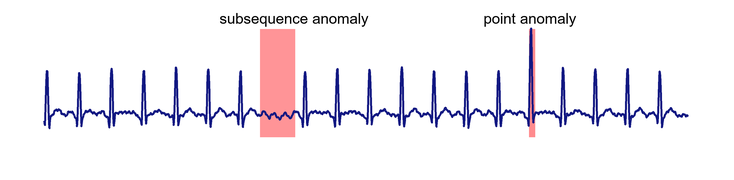
\includegraphics[width=0.78\textwidth]{figures/schmidl_anomaly_example.png}
    \caption{Example of point and subsequence anomalies in a time series \citep{schmidl2022anomaly}.}
    \label{fig:20}
\end{figure}




\section{Concept Drift}

Concept drift refers to a change in the underlying data distribution over time \citep{gama2014survey,lu2019learning}. In time-series data, this means that the definition of normal behavior is not fixed. A pattern that was unusual in the past may become normal later, or a previously normal pattern may disappear as the process evolves. Concept drift can appear in several forms.

% Abrupt drift occurs when the data changes suddenly from one normal pattern to another. For example, electricity usage may drop sharply between weekday and weekend. Gradual drift occurs when the transition happens slowly, such as seasonal temperature changes from winter to spring. Recurring drift occurs when a previously seen normal pattern returns, such as repeated daily, weekly, or seasonal shopping behavior.

\textcolor{blue}{Abrupt drift occurs when the data changes suddenly from one normal pattern to another. As shown in Figure~\ref{fig:211}(a), before the `sudden change point', the time series follows pattern A, and then rapidly switches to pattern B. This type of drift may occur when there is a significant change in electricity usage behavior between weekdays and weekends.}

\textcolor{blue}{When the transition from one normal pattern to another occurs slowly over a period of time, gradual drift occurs. Figure~\ref{fig:211}(b) illustrates this situation, where there is a transitional window between pattern A and pattern B. During this period, the signal may slowly shift from one behavior to another. A typical example is the seasonal change in temperature from winter to spring. The boundary between normal evolution and abnormal is unclear.}

\textcolor{blue}{Recurring drift refers to a previously observed normal pattern disappearing for a period of time and then reappearing later. As shown in Figure~\ref{fig:211}(c), this sequence initially follows pattern A, then changes to pattern B, and subsequently returns to pattern A. This situation can occur in daily, weekly, or seasonal behaviors, such as repetitive shopping patterns. This regressive pattern should be recognized as an effective normal pattern rather than a completely new anomaly.}



\begin{figure}[H]
    \centering
    \begin{tikzpicture}[
        x=0.85cm,
        y=0.85cm,
        >=Stealth,
        signal/.style={very thick, blue!70!black},
        oldregion/.style={fill=blue!7, draw=none},
        newregion/.style={fill=orange!12, draw=none},
        transitionregion/.style={fill=gray!15, draw=none},
        driftmark/.style={densely dashed, thick, red!70!black},
        paneltitle/.style={font=\bfseries\small, anchor=west},
        smalllabel/.style={font=\scriptsize}
    ]

    % a Abrupt drift
    \begin{scope}[shift={(0,8.5)}]
        \fill[oldregion] (0,0) rectangle (4.1,2.35);
        \fill[newregion] (4.1,0) rectangle (9.0,2.35);

        \draw[->] (0,0) -- (9.4,0) node[right,smalllabel] {Time};
        \draw[->] (0,0) -- (0,2.55) node[above,smalllabel] {Value};

        \draw[signal] plot[smooth] coordinates {
            (0.2,1.05) (0.9,1.32) (1.6,0.92) (2.3,1.25)
            (3.0,0.95) (3.7,1.18) (4.05,1.02)
        };
        \draw[signal] plot[smooth] coordinates {
            (4.15,1.78) (4.9,2.05) (5.6,1.68) (6.3,1.95)
            (7.0,1.72) (7.7,2.02) (8.5,1.82)
        };

        \draw[driftmark] (4.1,0) -- (4.1,2.35);
        \node[paneltitle] at (1,2.85) {(a) Abrupt drift};
        \node[smalllabel] at (2.0,2.15) {Pattern A};
        \node[smalllabel] at (6.6,2.15) {Pattern B};
        \node[smalllabel, red!70!black, align=center] at (4.1,-0.45) {sudden change point};
    \end{scope}

    % b Gradual drift
    \begin{scope}[shift={(0,4.2)}]
        \fill[oldregion] (0,0) rectangle (3.0,2.35);
        \fill[transitionregion] (3.0,0) rectangle (6.2,2.35);
        \fill[newregion] (6.2,0) rectangle (9.0,2.35);

        \draw[->] (0,0) -- (9.4,0) node[right,smalllabel] {Time};
        \draw[->] (0,0) -- (0,2.55) node[above,smalllabel] {Value};

        \draw[signal] plot[smooth] coordinates {
            (0.2,0.88) (0.9,1.12) (1.6,0.82) (2.3,1.05)
            (3.0,1.00) (3.7,1.18) (4.4,1.32) (5.1,1.50)
            (5.8,1.65) (6.5,1.78) (7.2,2.02) (7.9,1.74) (8.6,1.95)
        };

        \draw[driftmark] (3.0,0) -- (3.0,2.35);
        \draw[driftmark] (6.2,0) -- (6.2,2.35);
        \node[paneltitle] at (1,2.85) {(b) Gradual drift};
        \node[smalllabel] at (1.5,2.15) {Pattern A};
        \node[smalllabel] at (4.6,2.15) {transition window};
        \node[smalllabel] at (7.6,2.15) {Pattern B};
    \end{scope}

    % c Recurring drift
    \begin{scope}[shift={(0,0)}]
        \fill[oldregion] (0,0) rectangle (2.8,2.35);
        \fill[newregion] (2.8,0) rectangle (5.8,2.35);
        \fill[oldregion] (5.8,0) rectangle (9.0,2.35);

        \draw[->] (0,0) -- (9.4,0) node[right,smalllabel] {Time};
        \draw[->] (0,0) -- (0,2.55) node[above,smalllabel] {Value};

        \draw[signal] plot[smooth] coordinates {
            (0.2,1.00) (0.8,1.28) (1.4,0.90) (2.0,1.20) (2.6,1.02)
        };
        \draw[signal] plot[smooth] coordinates {
            (2.9,1.78) (3.5,2.03) (4.1,1.70) (4.7,1.98) (5.4,1.76)
        };
        \draw[signal] plot[smooth] coordinates {
            (5.9,1.02) (6.5,1.27) (7.1,0.92) (7.7,1.18) (8.5,1.00)
        };

        \draw[driftmark] (2.8,0) -- (2.8,2.35);
        \draw[driftmark] (5.8,0) -- (5.8,2.35);
        \node[paneltitle] at (1,2.85) {(c) Recurring drift};
        \node[smalllabel] at (1.4,2.15) {Pattern A};
        \node[smalllabel] at (4.3,2.15) {Pattern B};
        \node[smalllabel] at (7.4,2.15) {Pattern A};
    \end{scope}

    \end{tikzpicture}
    \caption{Three types of concept drift.}
    \label{fig:211}
\end{figure}

\reply{Draw tikzpicture for three types of drift, use the picture to illustrate, divide the three types into three paragraphs to expand this section}{Please see the blue texts above}
\fei{This is much too short given the importance of the topic.  You need to describe what is the difference between the three types of drift, and give examples.  Please expand.}

% \begin{figure}[H]
%     \centering
%     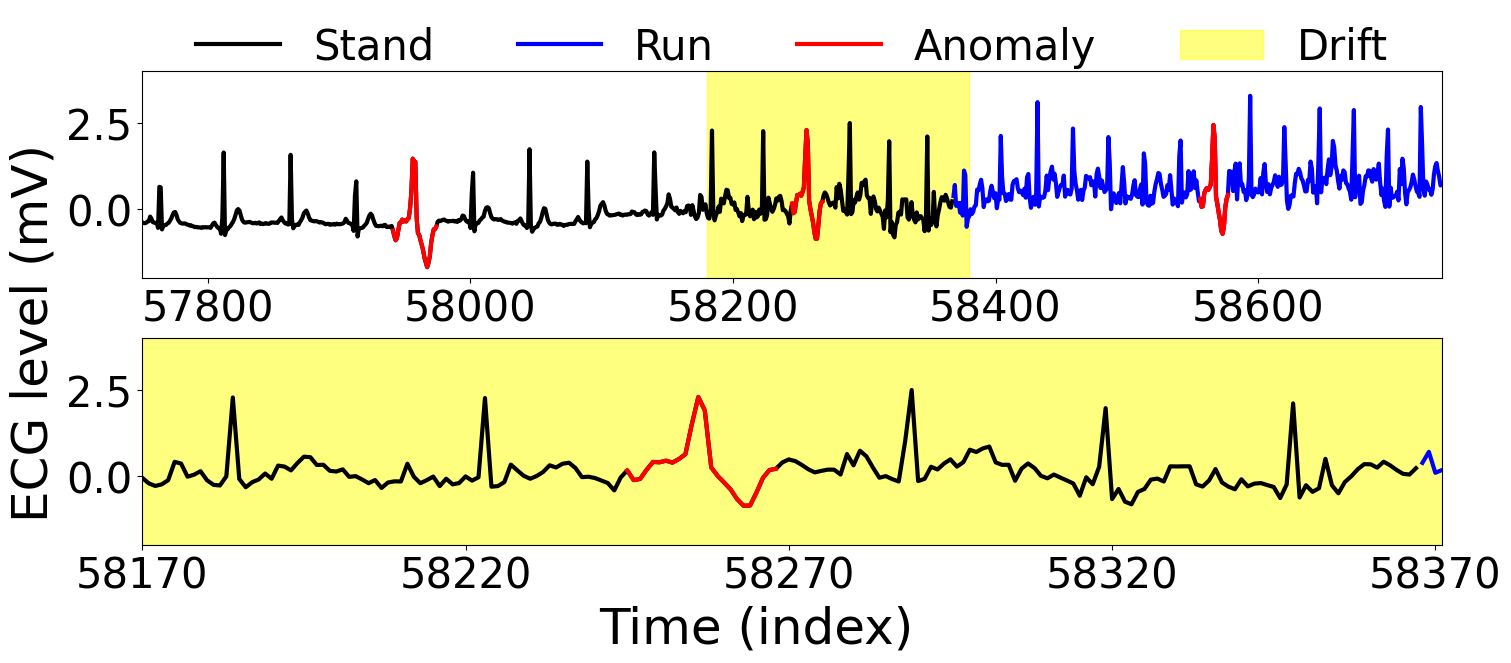
\includegraphics[width=0.85\textwidth]{figures/background_ecg_drift_anomaly.png}
%     \caption{Example of a time series containing both concept drift and anomalies. \citep{park2025adaptive}.}
%     \label{fig21}
% \end{figure}

\section{Normal Patterns}

\textcolor{blue}{The normal pattern refers to a representative subsequence or a group of similar subsequences used to describe the expected behavior in a time series. For example, in an electrocardiogram signal, a heartbeat cycle is generally regarded as one normal mode.}

\textcolor{blue}{Figure \ref{fig222} illustrates this concept using a simple time series. The red box marks a repetitive subsequence in the time series. These normal patterns follow the same structure. This repetitive segment represents the expected behavior in the data, so it can be classified as a normal pattern.}

\textcolor{blue}{The normal pattern is important for time series anomaly detection because new subsequences can be compared with known normal patterns. If a new subsequence is similar to an existing normal pattern, it is likely to be regarded as normal; if it differs significantly from all known normal patterns, it may receive a higher anomaly score. In data with concept drift, the set of normal patterns may also change over time: some patterns may become less active and new patterns need to be identified as normal patterns.}


\begin{figure}[H]
    \centering
    \begin{tikzpicture}[
        x=0.78cm,
        y=0.78cm,
        >=Stealth,
        base/.style={very thick, blue!70!black},
        pattern/.style={very thick, red!75!black},
        region/.style={fill=red!8, draw=red!60!black, rounded corners=2pt},
        smalllabel/.style={font=\scriptsize},
        titlelabel/.style={font=\bfseries\small}
    ]

    \draw[->] (0,0) -- (12.4,0) node[right,smalllabel] {Time};
    \draw[->] (0,0) -- (0,3.1) node[above,smalllabel] {Value};

    \fill[region] (4.6,0.12) rectangle (8.5,2.85);

    % Full time series
    \draw[base] plot[smooth] coordinates {
        (0.2,1.0) (0.7,1.15) (1.1,1.85) (1.55,2.35)
        (2.0,1.65) (2.45,0.95) (3.0,1.18) (3.6,1.05)
        (4.1,1.22) (4.6,1.10) (5.0,1.82) (5.45,2.30)
        (5.9,1.62) (6.35,0.98) (6.9,1.16) (7.5,1.02)
        (8.0,1.18) (8.5,1.12) (8.9,1.86) (9.35,2.32)
        (9.8,1.60) (10.25,0.94) (10.8,1.15) (11.4,1.04)
        (12.0,1.20)
    };

    \end{tikzpicture}
    \caption{Example of normal pattern in a time series.}
    \label{fig222}
\end{figure}

A normal pattern is a representative subsequence or group of subsequences that describes expected behavior in a time series. Many time-series anomaly detection methods compare a new subsequence against known normal patterns and treat large dissimilarity as evidence of abnormality.

\fei{This section is only two sentences and much too short to understand what is a normal pattern.  Please expand with more description and example.}
\reply{Draw a tikz picture to show normal pattern, expand this section}{Please see the blue texts above}

\section{Active Learning for User Feedback}

Active learning requests labels for selected uncertain data points instead of complete labels for all the dataset \citep{settles2009active}. This idea is related to human-in-the-loop machine learning, where human expertise is incorporated into the learning or decision-making process through feedback, correction, validation, or annotation \citep{amershi2014power,holzinger2016interactive}. The design is especially useful when fully automatic decisions are unreliable because the task requires domain knowledge. 

For anomaly detection with concept drift, partial user feedback is valuable because automatic scores alone may not fully determine whether a changed pattern is abnormal or newly normal. A user can confirm true anomalies, reject false positives, or validate candidate normal patterns. In this report, human feedback is used for refining anomaly thresholds and improving the distinction between abnormal events and drift-driven normal changes.